% Installed packages
\documentclass[tikz]{standalone}
\usepackage{comment}

% Tikz setup
\tikzset{>=latex}
\usetikzlibrary{matrix,shapes,arrows,arrows.meta,shadows,fit}

% Custom Tikz styles
\tikzstyle{block} = [draw, fill=gray!25, rectangle, minimum height=0.375in, minimum width=1in, semithick, rounded corners]
\tikzstyle{file} = [draw, fill=white, rectangle, minimum height=0.375in, minimum width=1in]
\tikzstyle{group} = [inner sep=7pt,draw,densely dashed,rounded corners]

\begin{document}

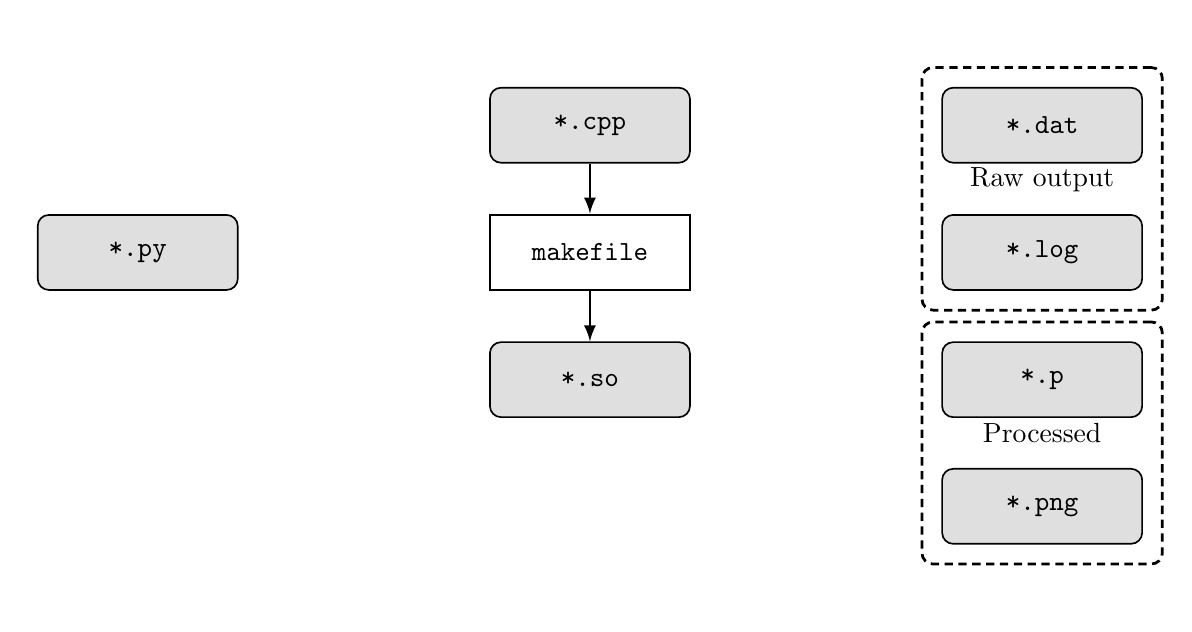
\begin{tikzpicture}[auto,node distance=2cm,font=\ttfamily,line width=1pt]

% Diagram nodes
\matrix[column sep=1.25in,row sep=0.25in]
{
	 & & \\
	 & \node[block](cpp){*.cpp}; & \node[block](dat){*.dat}; \\

	\node[block](py){*.py}; & \node[file](make){makefile}; & \node[block](log){*.log}; \\

	 & \node[block](so){*.so}; & \node[block](pickle){*.p}; \\

	 & & \node[block](png){*.png}; \\
	 && \\
};

% Draw connectors
\draw[->](cpp)--(make);
\draw[->](make)--(so);

% Group annotations
\node[group,fit=(dat)(log)]{\textrm{Raw output}};

\node[group,fit=(pickle)(png)]{\textrm{Processed}};

\end{tikzpicture}

\end{document}